\documentclass{article}
% translate with >> pdflatex -shell-escape <file>

% This file is an extract of the PGFPLOTS manual, copyright by Christian Feuersaenger.
% 
% Feel free to use it as long as you cite the pgfplots manual properly.
%
% See
%   http://pgfplots.sourceforge.net/pgfplots.pdf
% for the complete manual.
%
% Any required input files (for <plot table> or <plot file> or the table package) can be downloaded
% at
% http://www.ctan.org/tex-archive/graphics/pgf/contrib/pgfplots/doc/latex/
% and
% http://www.ctan.org/tex-archive/graphics/pgf/contrib/pgfplots/doc/latex/plotdata/

\usepackage{pgfplots}
\pgfplotsset{compat=newest}

\pagestyle{empty}

\begin{document}
\setlength{\fboxsep}{0pt}%
\fbox{%
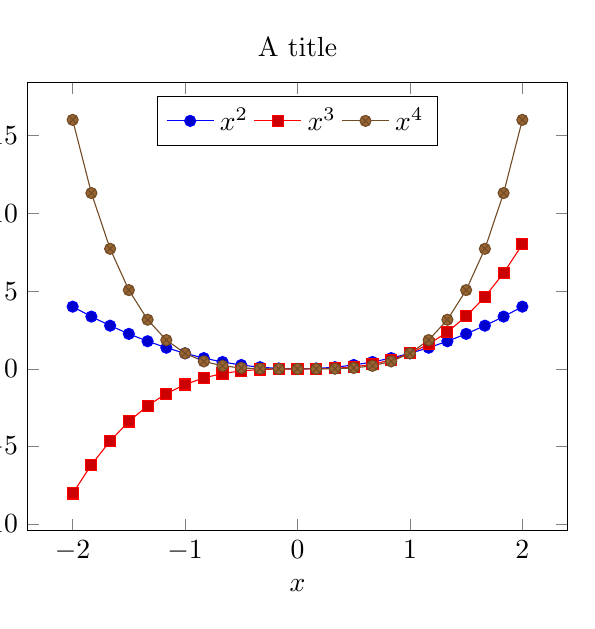
\begin{tikzpicture}%
	\begin{pgfinterruptboundingbox}
	\begin{axis}[
		title=A title,
		xlabel={$x$},
		ylabel={$y$},
		legend style={at={(0.5,0.97)},
			anchor=north,legend columns=-1},
		domain=-2:2
	]
	\addplot {x^2};
	\addplot {x^3};
	\addplot {x^4};
	\legend{$x^2$,$x^3$,$x^4$}
	\end{axis}
	\end{pgfinterruptboundingbox}

	\useasboundingbox 
			  (current axis.below south west)
	rectangle (current axis.above north east);
\end{tikzpicture}%
}%
\end{document}
